\chapter{Introduction}
\chaptermark{Introduction}

\section{Understanding the causes of variation in genetic diversity}

	\textit{``If we take the Darwinian view that evolution is the conversion of variation between individuals into variation between populations and species in time and space, then an essential ingredient in the study of evolution is a study of the origin and dynamics of genetic variation within populations''}\citep{RN183}

\noindent
This quote, from Lewontin's 1974 book \textit{The Genetic Basis of Evolutionary Change}, eloquently demonstrates that understanding the causes of variation between and within populations is one the central goals of evolutionary genetics, and has been for a long time.
	
	 In the latter half of the $20^{th}$ century, one of the foundational theories in population genetics was developed, the neutral theory of molecular evolution. The neutral theory contended that molecular changes between populations were predominantly the result of random changes in allele frequencies through time \citep{RN175}. In the past 30 years of population genetic research, the increasing availability of DNA sequence data has led to an understanding that neutral evolution cannot readily explain patterns of variability and between within species \citep{RN358}. However, an understanding of the factors that shape molecular variability in natural populations is far from complete.

	In this thesis, I describe three projects in which I have analysed different aspects of population genomic data from wild mice. Each project aims to increase our understanding of the factors shaping molecular variation in the genome. Wild mice are an excellent model system for studying molecular evolution in mammals for several reasons. Firstly, being one of the most well-studied organisms in all of science, the genomic resources developed for \textit{Mus musculus} are among the best available for any animal. Secondly, the size of wild mouse populations are very large, which results in high levels of genetic diversity (\textit{see below}), increasing power to statistical analyses. 

\section[Core concepts]{Core concepts in evolutionary genetics}

	Throughout this thesis I will refer to a number of fundamental concepts in population genetics. I give a brief description of several of these here.

\subsection{Genetic drift}

	In a finite population, the random sampling of individuals contributing to the next generation causes stochastic changes in allele frequencies. In a randomly mating, diploid population with non-overlapping generations of size \textit{N}, the probability that a new mutation, free from the effects of selection, goes to eventual fixation is simply its starting frequency, $\frac{1}{2N}$ (assuming autosomal inheritance). This implies that for any new, neutral mutation that arises, there is much larger probability, $1 - \frac{1}{2N}$, that it will be lost from the population. The change in allele frequency caused by random sampling is termed genetic drift. Genetic drift is very effective in small populations and less effective in large populations. As populations tend to infinite size, allele frequencies are not, on average, expected to change from generation to generation.
	
	The idealised population described above is referred to as a Wright-Fisher population. Natural populations obviously violate the assumptions of a Wright-Fisher population, for example humans have overlapping generations. In the above statement of the probability of fixation in the Wright-Fisher model, the census number of individuals ($N$) appeared. In order to model genetic drift for populations that violate the assumptions of the Wright-Fisher model, the effective population size ($N_e$) is used. Note that there is often a discrepancy between $N_e$ and $N$, for example the population undergoes inbreeding, $N_e$ is reduced by $N$. Natural selection is less effective if $N_e < N$ than in a Wright-Fisher population of size $N$ (see below) \cite{RN110}.

	Genetic drift does not operate solely on neutral alleles, indeed advantageous alleles may be lost through random sampling, but the probability of this depends on the selection coefficient (\textit{see below}).
	
\subsection{Neutrality and coalescence}

	The neutral theory of molecular evolution, proposed by Motoo Kimura, and later refined with Tamoka Ohta \citep{RN175}, posited that the vast majority of molecular evolution could be attributed to genetic drift with only a minority attributable to adaptation. In the strict sense, the neutral theory deals with mutations that are completely free from selective effects. A more relaxed definition, referred to as the \textit{nearly} neutral theory includes mutations that are weakly deleterious, such that their fates are predominantly decided by drift (\textit{see below}). Although tenets of the neutral theory have largely been shown to not hold in natural populations \citep{RN386, RN358, RN357}, the use of neutrality as a null hypothesis in molecular evolution has led to the development of a large number of statistical tests and the development of the coalescent.

	The coalescent is a framework for modelling molecular evolution that considers the evolutionary history of a sample of alleles drawn from a population. Working backwards in time, two alleles are said to \textit{coalesce} when they share a common ancestor at a particular time in the past. The probability of coalescence $t$ generations ago for a pair of neutrally evolving alleles is,
	\begin{equation}
	Pr(t) = \Big(1 - \frac{1}{2N}\Big)^{t-1}\frac{1}{2N}.
	\label{eq:coal}
	\end{equation}
\noindent
Equation \ref{eq:coal} is a geometric distribution, which, as $N \to \infty$ can be approximated by the continuous time exponential distribution. The rate parameter of this exponential distribution is $\lambda = \frac{1}{2N}$. Since the mean of the exponential distribution is the reciprocal of the rate parameter, the mean time to coalescence for a pair of randomly selected neutral alleles  when $N$ is large is simply $2N$.
		
\subsection{Population structure}

	The simplest population genetic models assume that the gametes that are sampled to produce progeny for the next generation behave like beans in a bag, where each bean has an equal probability of being sampled. Natural population do not necessarily behave like beanbags, however. Consider the case of an animal species that populates a long narrow range that stretches from North to South. Individuals at the top of the range, when seeking a mate, will be more likely to reproduce with an individual in their vicinity, rather than one from the South. Over time, this could lead to differences in allele frequencies along the North/South gradient. If one were to sequence individuals from across the range and perform a population genetic analysis on the resulting data that makes the assumption of a single randomly mating population, the differences in allele frequency due to the population structure could generate spurious results. The hypothetical example given above is relatively crude, true populations may be structured in very subtle (or in some cases not so subtle) ways that influence data analysis. Throughout this thesis, population structure is not analysed explicitly, but it is discussed as a potential confounding factor.

\subsection{Mutation and genetic diversity}

	Mutation is the ultimate source of all biodiversity. Mutation can be defined as a heritable change in an organism's genetic sequence. Mutations may occur during DNA repair, be affected by physical or chemical agents (e.g. UV radiation) or caused by errors in replication during meiosis or mitosis. There are numerous categories of mutations that have been described (e.g. translocations, inversions, insertions, deletions and point mutations). The most common of type of mutations, and the one most pertinent to this thesis, is single nucleotide substitution or point mutation. Point mutations involve the change of a single nucleotide from one of the four bases to another (e.g. adenine to cytosine). The rate of point mutation is higher than for small insertions and deletions, perhaps as much as an order of magnitude higher than for small insertion and deletions (e.g. \citealt{RN387}). Throughout this thesis I deal only with point mutations, unless otherwise stated.

	Depending on the population size, new mutations may be heavily influenced by genetic drift. The rate at which new mutations enter into the population obviously depends on population size, the more individuals there are, the more chances there are for mutations to occur. The probability that two randomly chosen individuals differ at a particular nucleotide in the genome depends on the time since they shared a common ancestor $t$. Working backwards along the two branches leading to the common ancestor, there is a total of $2t$ generations separating the two alleles. If the per site per generation mutation rate is $\mu$, then in the time separating two alleles, there is a probability of $2t$ that a mutation arose. As we saw above, the mean time to coalescence for pair of neutral alleles is $2N_e$, so the probability that two randomly chosen alleles differ is
	\begin{equation}
	\theta = 4N_e\mu. 		
	\end{equation}
\noindent
The average number of pair wise differences between sequences ($\pi$) therefore gives an estimate of the probability that two randomly chosen alleles differ in state, so $\pi$ can be used as an estimator of $\theta$. This quantity, $\pi$, or $\theta_{\pi}$ as it is sometimes denoted, is easily calculable from the polymorphism data. 


\subsection{Selection}

	The vast majority of the mouse genomes is not evolutionarily conserved, and thus can be inferred to be non-functional \citep{RN161}. Most mutations that occur will, therefore, not affect  their carriers' fitness. However, new mutations occurring in functional regions may be subject to selection. Throughout this thesis, I will refer to the selection coefficient ($s$), which is defined in terms of the relative fitnesses of the three genotypes possible at a biallelic locus, where $A$ is the wild-type allele and $a$ is the allele subject to selection:

\begin{center}
\begin{tabular}{c | c | c | c }
	Genotype & AA & Aa & aa \\ \hline
	Fitnesses& $1$ & $1 + sh$ & $1 + s$ \\
\end{tabular}
\end{center}	

\noindent

Here, $h$ is the dominance coefficient of new mutations; under additivity $h = 0.5$,  complete dominance $h = 1$, complete recessivity $h = 0$, and heterozygote advantage $h > 1$. In this thesis, selected mutations are assumed to behave additively, unless otherwise stated. 

	Even when selection is acting on a new mutation, genetic drift may still operate. As derived by both \cite{RN399} and \cite{RN199}, the fixation probability for a semi-dominant mutation with selective effect $s$, segregating at a frequency of ($q$) in a population of size $N_e$ is,

\begin{equation}
	u(s, N_e, q) = \frac{1 - e^{-2N_esq}}{1 - e^{-2N_es}}
	\label{eq:fixation}
\end{equation}

\noindent
In a Wright-Fisher population, the frequency of a new mutation is $\frac{1}{2N}$, so the exponent in the left-hand side of the numerator in Equation \ref{eq:fixation} is $\approx s$. From Equation \ref{eq:fixation}, it can be observed that the fixation probability of a new mutation is dependant on the relative magnitude of $N_e$ and $s$. If $N_e$ were large and the mutation were advantageous, the denominator $(1 - e^{-2N_es}) \to 1$, so $u(s, N_e, q) \approx s$. If the product $N_es \gg 1$, then the mutation behaves deterministically. In the case of deleterious mutations, (where $s < 0$), if $|N_es| > 1$ then $u(s, N_e, q) \to 0$.  For both advantageous and deleterious mutations if $|N_es| \leq 1$, then the fate of the mutation is similar to that of a neutral allele and genetic drift dominates. The factors that can affect $N_e$ (e.g. inbreeding, sex structure and population structure) cause a reduction in the efficacy of selection. If the effective population size, $N_e$, fell below the census size, $N$, then the fixation probabilities for strongly beneficial mutations will be reduced by a factor $N_e/N$.

	Throughout this thesis I frequently use the term neutral to describe molecular evolution dominated by genetic drift, including cases where $s << \frac{1}{2N_e}$

\subsection{The McDonald-Kreitman test}

	One of the most widely used methods for the detection of positive selection is the McDonald-Kreitman (MK) test \citep{RN293}. The MK-test contrasts molecular variation at putatively neutral sites with variation at potentially selected sites. Typically, synonymous and nonsynonymous sites in protein-coding genes are used as the neutral and selected site categories, respectively. Under the neutral theory, differences between species accumulate by the random fixation of neutral  alleles due to drift, with a negligible contribution from positive selection. As such, the ratio of nucleotide diversity at nonsynonymous/synonymous sites ($\pi_N / \pi_S$) should be statistically indistinguishable from the ratio of nonsynonymous/synonymous divergence ($d_N / d_S$). An elevation of $d_N / d_S$ above the value expected given $\pi_N / \pi_S$ is taken as evidence for positive selection. The MK-framework has been expanded to allow the estimation of the proportion of nucleotide substitutions at a particular class of sites, driven by positive selection ($\alpha$)

\begin{equation}
\alpha = 1 - \frac{d_N \pi_N}{d_S \pi_S}.
\end{equation}
\noindent
\citep{RN294}. However, since weakly deleterious mutations at, for example, nonsynonymous sites may segregate in a population, estimates of $\alpha$ obtained in this way are likely underestimates. Further developments of the MK-test have been made that estimate the distribution of fitness effects for new mutations and use this to correct for the contribution deleterious mutations make to both standing variation and between-species divergence when performing MK-type analyses \citep{RN165}. 

\subsection{Recombination}

	Recombination is a fundamental process in the evolution of sexual organisms. Recombination involves the transfer of information from one chromosome copy to another via crossing over, the reciprocal exchange, or swapping, of DNA between homologous chromosomes, or gene conversion, where there is a non-reciprocal exchange between homologous chromosomes. In mammals, recombination is integral to the successful segregation of chromatids during meiosis. If recombination is suppressed, there are far higher rates of aneuploidy and other meiotic errors \citep{RN388}. During meiotic prophase, after the pairing of homologous chromosomes, a series of double-strand breaks (DSBs) are formed in each of the four chromatids \citep{RN388}. DSBs are typically resolved in two ways, one that predominantly leads to crossovers and one that leads to gene conversions. In mice, PRDM9 is a zinc-finger DNA-binding enzyme that recruits the protein complex that initiates DSBs \citep{RN388}. In many organisms crossing-over events typically occur in narrow genomic windows, referred to as recombination hotspots, and in mice these are enriched for the bindings motifs of PRDM9 \citep{RN388}.

	Recombination is an important process in evolution and is thought to provide a substantial benefit to sexual reproduction. There are numerous theories as to why meiotic recombination evolved, which can be summarised as a) preventing selective interference, resulting in more efficient responses to selection b) providing a moving evolutionary target to parasites by generating new genotype combinations and c) breaking apart harmful combinations of alleles \citep{RN389}. Genetically linked sites do not evolve independently, selection acting at one may have consequences for another. Because of this, the rate of recombination influences the consequences of natural selection.

\section[Models of selective sweeps]{Models of selective sweeps}

\cite{RN124} showed that an advantageous mutation drags with it linked neutral polymorphisms as it rises in frequency. With increasing genetic distance from the selected site, the effect is reduced, resulting in troughs in genetic diversity in surrounding regions.
 
 \begin{figure}[h!]
   \centering      
   \noindent\makebox[\textwidth]{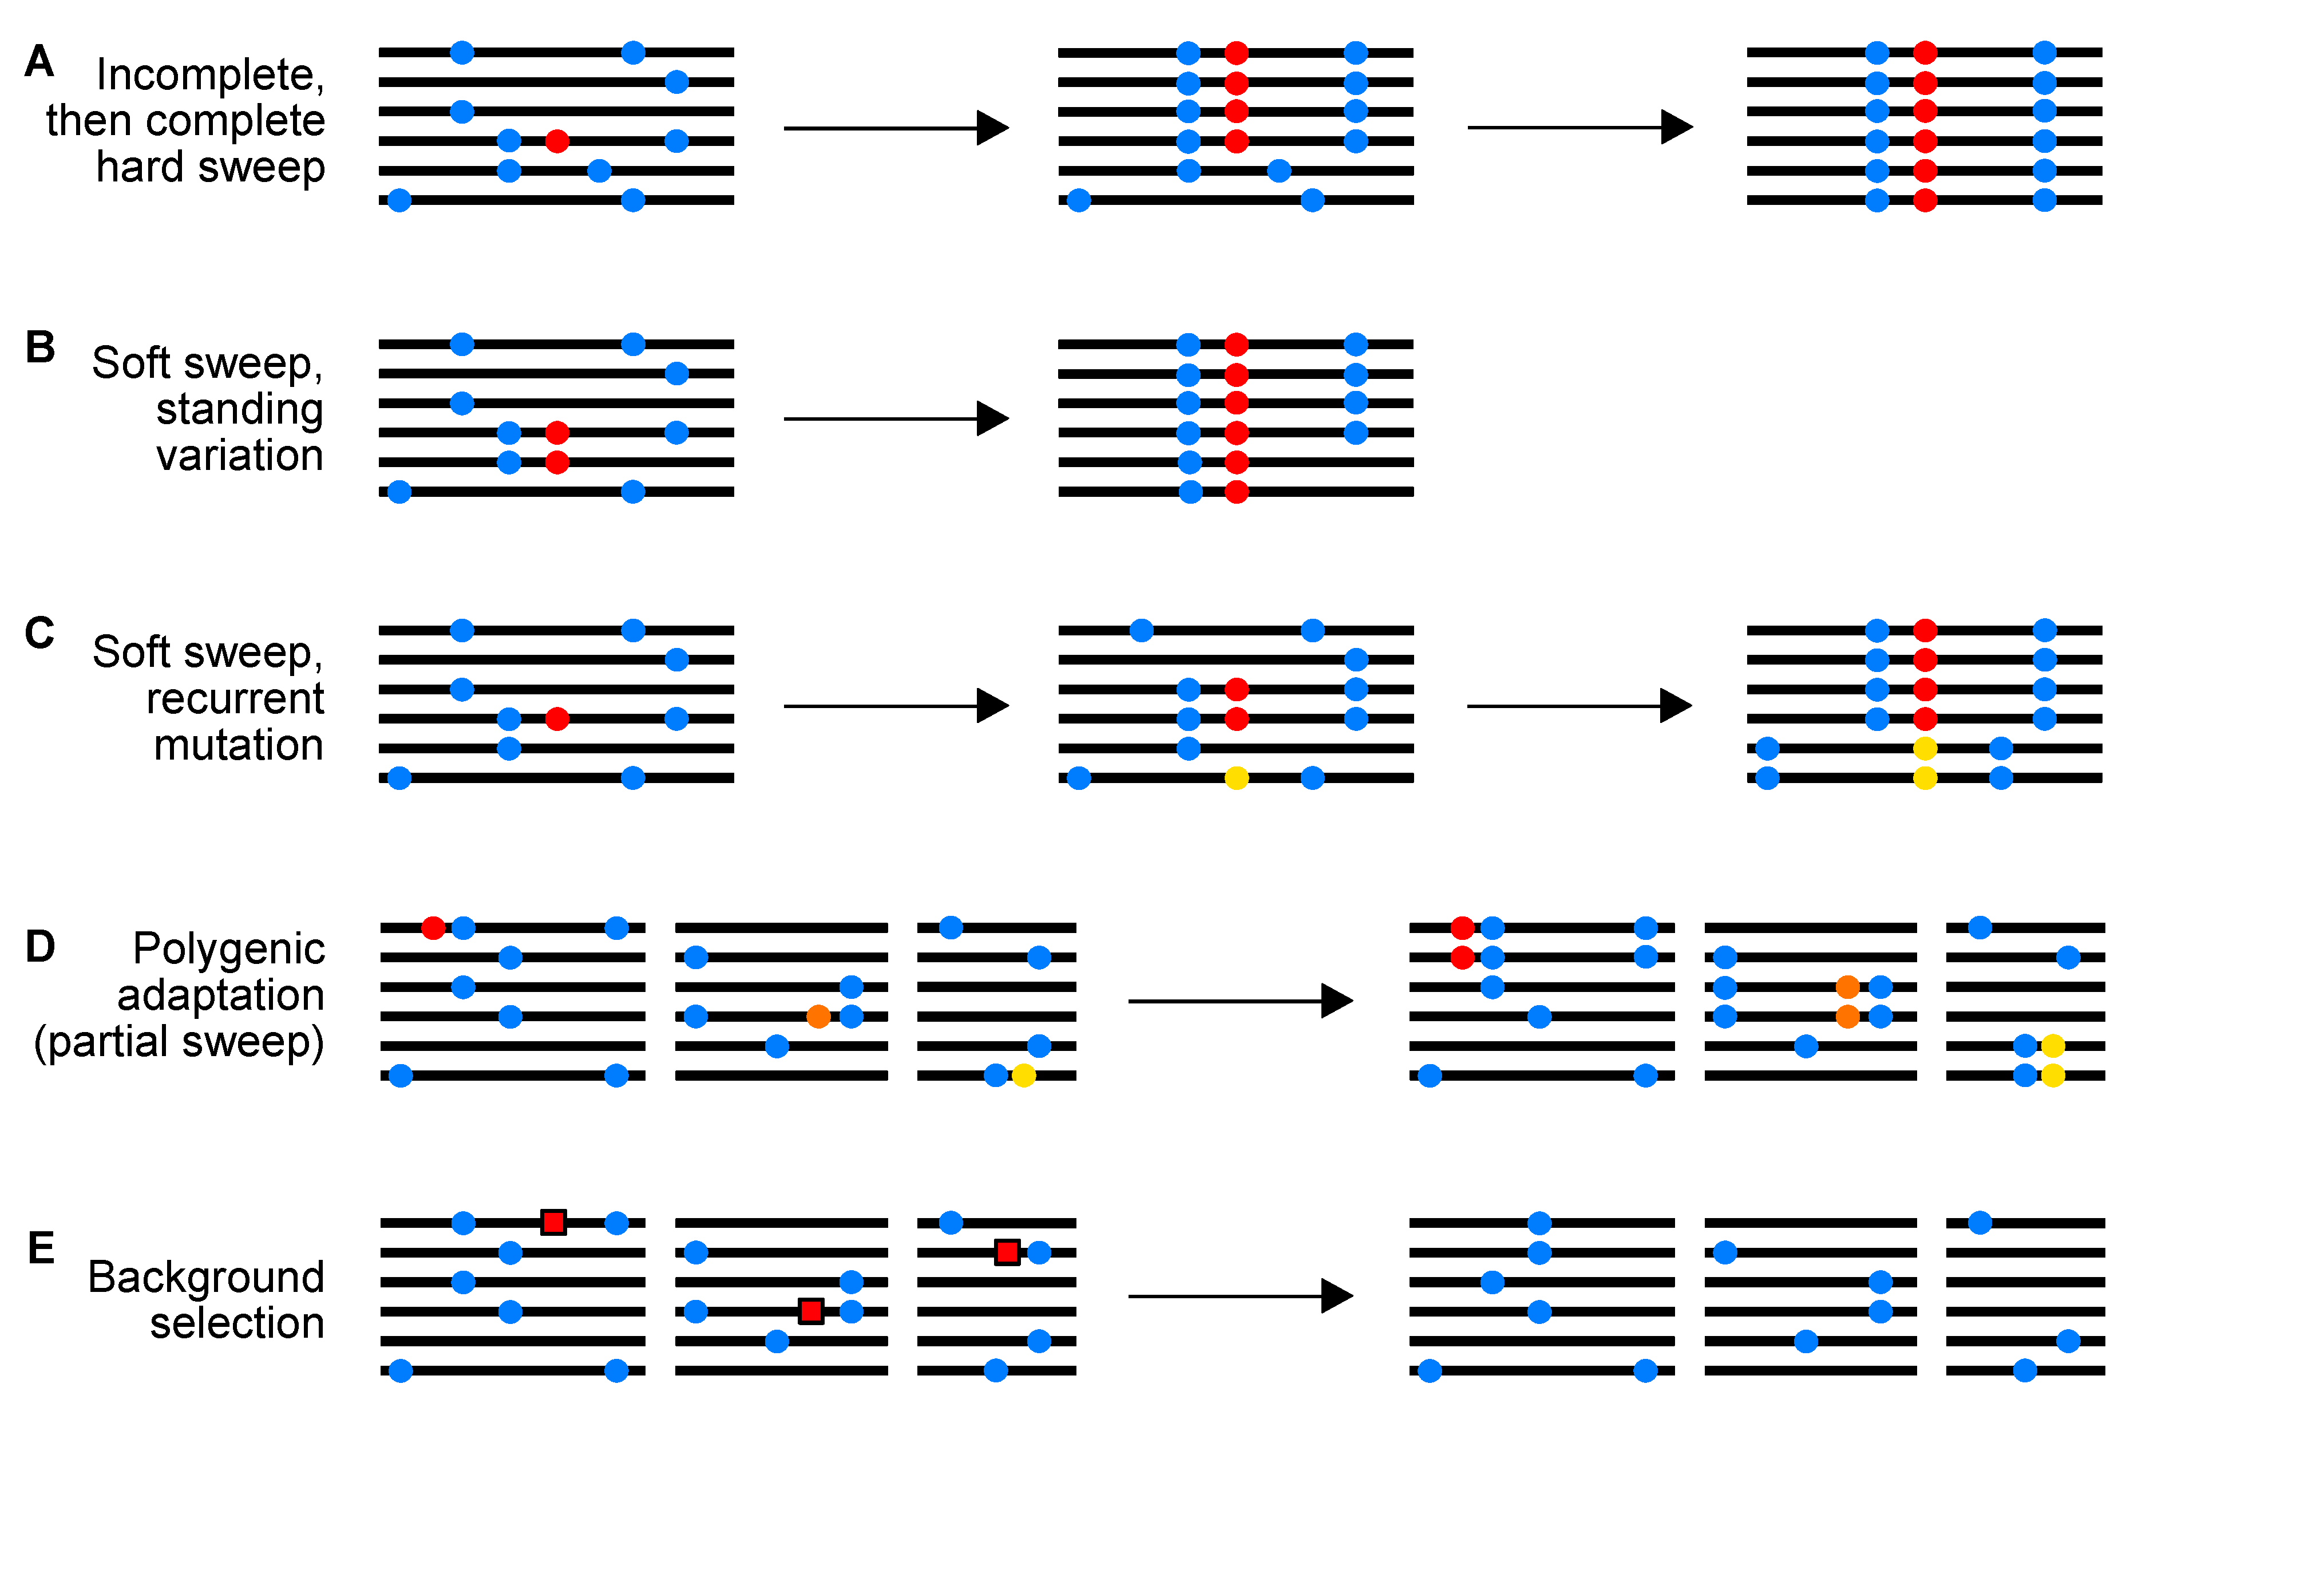
\includegraphics[width=\textwidth]{/Users/s0784966/Dropbox/Thesis/chapter1/figure_sweeps_no_legend.pdf}}
 \caption[Selective sweeps and background selection]{Selective sweeps and background selection. Blue circles represent neutral alleles, red, yellow and orange circles represent advantageous alleles, and red squares represent deleterious alleles. Reproduced from \cite{RN352}, courtesy of Ben Jackson.}.
 
 \label{fig:sweepCartoon}
\end{figure}


\subsubsection{Hard/classic sweeps} 
 
The most well-studied model of sweeps. A new advantageous mutation rapidly increases in frequency to eventual fixation (shown in Figure \ref{fig:sweepCartoon}-A). As it sweeps, the adaptive allele carries with it a portion of the haplotype on which it arose, reducing levels of neutral diversity in the surrounding area \citep{RN124,RN235}. 
 
\subsubsection{Soft sweeps} 
  
A neutral allele segregating in a population may become favoured (due, for example, to a change in the environment). The segregating allele may be associated with multiple haplotypes, and as it rises in frequency, so do the multiple haplotypes (shown in \ref{fig:sweepCartoon}-B). A similar process, also termed a soft sweep, can occur if an advantageous mutation arises by multiple, distinct mutation events (shown in \ref{fig:sweepCartoon}-C). 
 
\subsubsection{Incomplete/partial sweeps} 
 
If an advantageous allele increases in frequency, but does not reach fixation, there will still be some loss of linked neutral diversity. In this review we use the term incomplete sweeps to describe sweeps that are polymorphic at the time of sampling, but may (or may not) eventually reach fixation (shown in \ref{fig:sweepCartoon}-A). The term partial sweep describes the situation wherein a sweeping allele becomes effectively neutral at a certain frequency in its trajectory (shown in \ref{fig:sweepCartoon}-D). The magnitude of both processes on linked neutral diversity depend on the frequency reached by the sweeping allele when selection is ‘turned off’ or on the time of sampling \citep{RN226}. Partial sweeps may be common in cases of adaptation involving selection on quantitative traits \citep{RN147}. 

\subsection{Background selection} 
As natural selection purges deleterious mutations, neutral alleles linked to the selected locus are also lost. The process of background selection is qualitatively similar to recurrent selective sweeps, since both processes reduce local genetic diversity \citep{RN110} and skew the site frequency spectrum towards rare variants \citep{RN287, RN113}. Models of background selection envisage a neutral site linked to many functional sites at different distances, such that the effects of selection at many sites accumulate to reduce diversity \citep{RN206,RN157}. 

\section[Using models of selective sweeps to estimate positive selection parameters]{Using models of selective sweeps to estimate positive selection parameters}
 
Population geneticists have long sought to understand the contribution of natural selection to molecular evolution. A variety of approaches have been proposed that use population genetic theory to quantify the rate and strength of positive selection acting in a species’ genome. In the following section, I discuss methods that use patterns of between-species nucleotide divergence and within-species diversity to estimate positive selection parameters from population genomic data. We also discuss recently proposed methods to detect positive selection from a population’s haplotype structure. The application of these tests has resulted in the detection of pervasive adaptive molecular evolution in multiple species.
 
If adaptive substitutions are common, selection is expected to leave footprints in genetic diversity at linked sites. In particular, as a positively selected mutation increases in frequency, it tends to reduce diversity at linked neutral loci. Theoretical analysis of this process, termed a selective sweep (\textit{see above}), has shown that the reduction in diversity at a linked neutral locus depends on the ratio of the strength of positive selection to the recombination rate. Thus, comparing diversity at multiple neutral loci linked to selected regions, in principle, should provide an indirect means for estimating parameters of positive selection.

If a population experiences recurrent selective sweeps, there are several patterns predicted by theory. Under recurrent hard selective sweeps, levels of genetic diversity are expected to be lower i) in regions of the genome with restricted recombination, ii) in regions experiencing many sweeps and iii) in the genomic regions surrounding the targets of selection themselves. Each of these of these predictions have been met in empirical studies, and each has been used to estimate parameters of positive selection.

\subsection[The correlation between diversity and the rate of recombination]{The correlation between diversity and the rate of recombination}

In the late 1980s, evidence began to emerge suggesting that genetic polymorphism are less frequent in genomic regions experiencing restricted crossing-over \citep{RN225,RN282}. Soon after, \cite{RN114} showed that there is a positive correlation between nucleotide diversity and the rate of crossing-over in \emph{D. melanogaster}, a pattern subsequently observed in other eukaryotic species \citep{RN117}. Begun and Aquadro pointed out that the correlation is qualitatively consistent with the action of recurrent selective sweeps. \cite{RN277} formulated expressions, based on the correlation between nucleotide diversity and the rate of recombination, to estimate the compound parameter $\lambda 2N_{e}s$, where $\lambda$ is the rate of sweeps per base pair per generation, $N_e$ is the effective population size and $s$ is the selection coefficient. They applied their method to the data of \cite{RN114}, estimating $\lambda2N_{e}s$ = 5.37 x $10^{-8}$, but their method could not disentangle the individual parameters. More recently, \cite{RN226} performed a similar analysis in \emph{D. melanogaster} to explore the effects of partial sweeps on parameter estimates. They showed that when partial sweeps are common, the rate of adaptive evolution is underestimated if the hard sweep model is assumed.
 
The correlation between diversity recombination observed by \cite{RN114} can also be explained by background selection, the reduction in neutral diversity caused by the removal of linked deleterious mutations \citep{RN132}. The process of background selection is qualitatively similar to recurrent selective sweeps, since both processes reduce local genetic diversity \citep{RN110} and skew the SFS towards rare variants \citep{RN287,RN133}. Models of background selection envisage a neutral site linked to many functional sites at different distances, such that the effects of selection accumulate to reduce diversity \citep{RN206, RN157}. The correlation between neutral diversity and the recombination rate predicted by background selection is quantitatively similar to that observed in \emph{D. melanogaster} \citep{RN281}. Indeed, recent studies suggest that background selection is a major determinant of nucleotide diversity variation at broad scales ($>$100Kbp) in humans \cite{RN120} and \emph{D. melanogaster} \citep{RN288, RN116}. It is clear, then, that background selection is a key confounding factor when attempting to make inferences about positive selection.
 
\subsection[Correlations between neutral diversity and non-neutral divergence]{Correlation between neutral diversity and non-neutral divergence}

If there is a constant fraction of adaptive substitutions, $\alpha$, across the genome for a given class of sites, regions that evolve at higher rates should experience a greater number of selective sweeps. Under a model of recurrent sweeps, it follows that there should be a negative correlation between nucleotide divergence at selected sites and diversity at linked neutral sites. This was first described in \textit{Drosophila melanogaster} by \cite{RN283}, and has been subsequently reported in other \textit{Drosophila} species \citep{RN284}. Assuming a single rate of sweeps ($\lambda$) and a constant scaled strength of positive selection ($2N_es$) for a given class of sites, \cite{RN283} generalised formulae of \cite{RN277} based on the correlation between synonymous site diversity and non-synonymous site divergence to estimate  $\lambda 2N_es$ = $3 \times 10^{-8}$ for the X-chromosome in \textit{D. melanogaster}. Note that this $\lambda 2N_es$ estimate is similar to that obtained based on the correlation of synonymous site diversity and recombination rate (\cite*{RN277}; see above). Using an estimate of $\alpha = 0.50$ obtained from a MK-based analysis, \cite{RN283} decomposed the $\lambda 2N_es$ compound parameter, and inferred that $s \approx 0.001\%$ and $\lambda$ = $3.6 x 10^{-11}$ /bp/generation, suggesting that adaptation of protein-coding genes in \textit{D. melanogaster} is driven by moderately weak selection (i.e., assuming \textit{D. melanogaster} $N_e =10^6$, $2N_es \approx 40$). In a related study, \cite{RN289} estimated $\lambda 2N_es \approx 10^{-7}$ in \textit{D. simulans}, also by examining the correlation between mean neutral diversity and selected (nonsynonymous) divergence. However, their model also included the heterogeneity in levels of diversity, which is related to the rate and strength of sweeps in a different way to the mean, and allowed the individual parameters to be fitted by regression. The estimates of the compound parameter $\lambda 2N_es$ are similar between the two studies, though \cite{RN289} estimated that $s \approx 1\%$ (compared to Andolfatto’s estimate of $s \approx 0.001 \%$) and $\lambda = 3.6 \times 10^{-12}$ /bp/generation. The discrepancies between the studies may be due to differences in biology between the species, or may reflect methodological differences: For example, if the majority of adaptive substitutions are driven by weakly selected sweeps, which will leave a relatively small signal in levels of  polymorphism, the MK-based method may more sensitively detect them, perhaps explaining the higher rate of sweeps inferred by \cite{RN283}. On the other hand, strongly selected sweeps will leave a larger footprint in levels of diversity, so will be more readily detected using the approach of \cite{RN289}, perhaps explaining why they inferred a lower overall rate of sweeps, with higher selection coefficients (for a full description, see \citealt{RN171}). In both cases, inferences based on variation in polymorphism may reflect processes other than the fixation of adaptive alleles that have gone to fixation, such as partial sweeps and background selection, as these will affect patterns of diversity but not necessarily divergence. Related to this, the approach employed by \cite{RN283} has recently been extended by \cite{RN323}, by estimating the correlation between synonymous site diversity and non-synonymous divergence in the presence of both background selection and gene conversion in \textit{D. melanogaster}. They found that ignoring background selection tends to increase and decrease estimates of selection strength and rate, respectively. The parameter values estimated in their study suggest that 0.02\% of new mutations at nonsynonymous sites are strongly selected ($s \approx 0.03\%$, assuming $N_e$ = $10^6$ for \textit{D. melanogaster}).
 
\subsection[Patterns of diversity around the targets of selection]{Patterns of diversity around the targets of selection}
 
An individual hard selective sweep is expected to leave a trough in genetic diversity around the selected site. If a large proportion of amino acid substitutions are adaptive, as suggested by MK-type analyses (see \citealt{RN215}), collating patterns of diversity around all substitutions of a given type should reveal a trough in diversity. Such a pattern is not expected around a “control” class of sites, such as synonymous sites. This test, proposed by \cite{RN167}, was first applied it to \textit{D. simulans}, and the above pattern was found. By fitting a hard sweeps model to the shape of the diversity trough, they estimated α values of  5\% and 13\%, depending on whether one or two classes of beneficial mutational effects were fitted. Note that their estimates of α are substantially lower than those obtained using MK-based methods for \textit{D. melanogaster} \citealt{RN283}. \cite{RN167} suggested that modes of selection other than hard sweeps may help explain to this discrepancy. However, even when modelling two classes of beneficial mutations, they found that amino acid substitutions are driven by strongly adaptive mutations ($s$ $sim0.5\%$ and $s$ $\sim0.01\%$). Their estimates of selection strength are therefore in broad agreement with the estimate of s $sim1\%$ obtained by \cite{RN289}, based on the correlation between synonymous diversity and non-synonymous divergence in \textit{D. simulans}. The \cite{RN167} test, then, suggests that adaptation in protein-coding genes is fairly frequent and driven by strong, hard sweeps.
 
The Sattath test has been applied in a variety of organisms, including humans \citep{RN162}, wild mice \citep{RN122}, \textit{Capsella grandiflora} \citep{RN236} and maize \citep{RN230}. In all but \textit{C. grandiflora}, researchers have found no difference in patterns of diversity around selected and neutral substitutions. These results have been interpreted as evidence that hard sweeps were rare in the recent history of both humans \citep{RN162} and maize \citep{RN230}. However, \cite{RN237} pointed out that the Sattath test will be underpowered if there is large variation in levels of functional constraint in the genome. Indeed, through their analyses \cite{RN237} found evidence for frequent adaptive substitutions in humans, particularly in regulatory sequence. To address the issues raised by \cite{RN237}, \cite{RN230} applied the Sattath test to substitutions in maize genes with the highest and lowest levels of functional constraint separately, but still found no difference in diversity pattern, suggesting either that hard sweeps have been rare in that species or that there is another confounding factor.
 
One possible explanation is that the species in which the Sattath test did/did not detect hard sweeps have distinct patterns of linkage disequilibrium (LD). LD decays to background levels within hundreds of base-pairs in \textit{D. simulans} \citep{RN283} and \textit{C. grandiflora} \citep{RN271}, whereas in humans, maize and wild mice it decays over distances closer to 10,000bp \citep{RN273,RN327, RN272}. It may be, then, that the Sattath test is only applicable when there is relatively short-range LD, such that the patterns of diversity around selected substitutions do not substantially overlap with the analysis windows around neutral ones. If this were the case, interpreting the similarity in troughs of diversity around selected and neutral substitutions as evidence for a paucity of hard selective sweeps may not be justified in organisms where LD decays over distances of a similar order of magnitude as the width of the diversity troughs themselves.
   	        	  
\section[Fitting genome wide patterns]{Fitting genome wide patterns}

	Methods to estimate the rate and strength of positive selection in the genome employ various combinations of nucleotide diversity, divergence, recombination rates and estimates of background selection effects as summary statistics, averaged over many regions of the genome. Recently, \cite{RN274} developed a method that fits a model of hard sweeps and background selection to genome-wide variation in nucleotide diversity and divergence (at both selected and neutral sites). In \textit{D. melanogaster}, they showed that hard sweeps can explain a large amount of genome-wide variation genetic diversity. For nonsynonymous sites, they found that $\alpha = 4.1\%$ for strongly selected mutations ($s \geq 0.03\%$) and $\alpha = 36.3\%$ for weakly selected mutations ($s \approx 0.0003\%$), summing to $\alpha = 40.4\%$, which is similar to the estimate obtained using the MK-test \citep{RN283}. Their results suggest that accounting for weakly selected mutations may help reconcile the discrepancy between MK-based estimates of the rate and strength of selection and parameters estimated from sweep model predictions, described above.

\cite{RN274} showed that a map of the effects of hard sweeps and background selection is capable of explaining a large amount of the variation in diversity across the genome, further demonstrating that the action of natural selection is pervasive, at least in \textit{D. melanogaster}. However, their method overestimated the rate of deleterious mutations, which the authors attribute to the presence of modes of adaptation other than hard sweeps in \textit{D. melanogaster}. 

\section[\cite{RN122}]{\cite{RN122}}


	The research I have performed throughout my PhD carries on from the work of \cite{RN122}, it is fitting, therefore, to give a brief description of the key findings from that study.
	
	\cite{RN122} sequenced the genomes of 10 wild-caught \textit{Mus musculus castaneus} individuals, using high-throughput sequencing methods. They sequenced individuals to high coverage, using multiple libraries of Illumina paired-end reads. Based on an analysis of population structure, the individuals sequenced were thought to represent a single admixed group. \cite{RN122} extracted polymorphism data from genomic regions surrounding both protein-coding exons and conserved non-coding elements (CNEs - which were inferred to be involved in gene regulation), and found dips (or troughs) in average diversity surrounding the elements themselves. As discussed above, \cite{RN122} applied the Sattath analysis to their data, but found that there was no difference in the average diversity around nonsynonymous/synonymous substitutions. They also modelled the contribution BGS made to the troughs in diversity around both protein-coding exons and CNEs using a population genetic model, and found that it could not fully explain the observed patterns of diversity. Our understanding of the factors that shape nucleotide diversity across the mouse genome are, thus, somewhat unclear.

\section[Thesis aims]{Thesis aims}

	The aim of this thesis is to further our understanding of the factors that shape variation in genetic diversity across the mammalian genome using the house mouse as a model. Particularly, I focus on the contributions of background selection and selective sweeps to variation in genetic diversity across the mouse genome. 

	\begin{itemize}
	
	\item In Chapter 2, I leverage information from patterns of linkage disequilibrium across the mouse genome to construct recombination rate maps for the mouse genome. I use these to investigate the relationship between nucleotide diversity and recombination rate. 
	
	\item In Chapter 3, I estimate the distribution of fitness effects both advantageous and deleterious mutations for multiple classes of sites in the mouse genome. I use these estimates to parametrise forward-in-time population genetic simulations. By analysing these simulations, I attempt to dissect the contributions of selective sweeps and background selection to troughs in diversity around functional elements.
	
	\item In Chapter 4, I fit a model incorporating the effects of selective sweeps and background selection to troughs in diversity around functional elements in mice. Using the parameters that provide the best fit to the data, I ask whether adaptation in protein-coding or  regulatory regions contributes most to fitness change in mice.
	
	\end{itemize}

